\chapter{Введение}
В данной работе был использован фреймворк Mr.LDA\cite{mrlda}, который основывается на модели Латентного 
размещения Дирихле (LDA).

Модель LDA решает классическую задачу анализа текстов: создать вероятностную модель большой 
коллекции текстов.

Очевидно, что у одного документа может быть несколько тем; подходы, которые кластеризуют документы по 
темам, никак этого не учитывают. LDA -- это иерархическая байесовская модель, состоящая из двух уровней:
\begin{itemize}
    \item на первом уровне -- смесь, компоненты которой соответствуют <<темам>>;
    \item на втором уровне -- мультиномиальная переменная с априорным распределением Дирихле, 
        которое задаёт <<распределение тем>> в документе.
\end{itemize}

\begin{figure}
    \center
    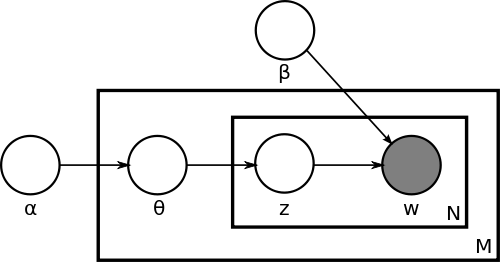
\includegraphics[width=0.47\textwidth]{lda}
    \caption{Граф модели}
\end{figure}

Сложные модели часто проще всего понимать рассмотрев на примере как модель будет генерировать новый 
документ:
\begin{itemize}
    \item выбрать длину документа \( N \) (этого на графе не нарисовано -- это не то чтобы часть модели);
    \item выбрать вектор \( \theta \sim (\alpha) \) -- вектор <<степени выраженности>> каждой темы в 
        этом документе;
    \item для каждого из \( N \) слов \( w \):
    \begin{itemize}
        \item выбрать тему \( z_n \) по распределению \( Mult(\theta) \);
        \item выбрать слово \( w_n \sim p(w_n | z_n, \beta) \) с вероятностями, заданными в \( \beta \).
    \end{itemize}
\end{itemize}

Для простоты мы фиксируем число тем \( k \) и будем считать, что \( \beta \) -- это просто набор параметров
\( \beta_{i,j} = p(w^j = 1 | z^i = 1)\), которые нужно оценить. Совместное распределение тогда выглядит так:
\[
    p(\theta,\ldots,N|\alpha,\beta) = 
        p(N|\eta)p(\theta|\alpha)\prod\limits_{n=1}^{N}p(z_n|\theta)p(w_n|z_n,\beta)
\]
В отличие от обычной кластеризации с априорным распределением Дирихле или обычного наивного байеса, мы 
тут не выбираем кластер один раз, а затем накидываем слова из этого кластера, а для каждого слова 
сначала выбираем по распределению \( \theta \) тему, а уже потом набрасываем это слово по этой теме.

На выходе после обучения модели LDA получаются векторы \( \theta \), показывающие, как распределены темы в 
каждом документе, и распределения \( \beta \), показывающие, какие слова более вероятны в тех или иных 
темах. Таким образом, из результатов LDA легко получить для каждого документа список встречающихся в нём 
тем, а для каждой темы -- список характерных для неё слов, то есть фактически описание темы.\cite{lda}

\chapter{Получение информации}
Были получены указания разобраться с работой фреймворка Mr.LDA и обучить классификатор для работы 
с патентными документами. Также были получены следующие документы:
\begin{itemize}
    \item отчёты и другие документы по проделанной работе ранее;
    \item frontend на Scala для работы с классификатором;
    \item исходные коды для работы с Mallet;
    \item выборка патентных документов состоящая из \(\sim 15\) тысячи документов.
\end{itemize}

\chapter{Установка ПО}
Так как пока нет возможности получить доступ к оборудованию, на котором будет проводиться работа с 
патентными документами, то установка необходимого программного обеспечения была произведена на 
собственном стационарном компьютере.

В качестве операционной системы для работы выбрать Arch Linux\cite{arch}, так как она уже была 
установлена на рабочем компьютере. Для этой ОС есть все последние версии пакетов программ.

На рабочую систему были установлены следующие программные компоненты:
\begin{itemize}
    \item Java Development Kit (jdk7-openjdk 7.u71\_2.5.3-1);
    \item Scala 2.11.4-1;
    \item Apache Hadoop 2.5.2-1;
    \item Python 3.4.2;
\end{itemize}
А также дополнительные компоненты, идущие в зависимостях у этих пакетов.

\chapter{Конфигурация ПО}
Конфигурация фреймворка Apache Hadoop была выполнена с помощью дополнительной литературы из 
вики\cite{archwiki} по ссылке \url{https://wiki.archlinux.org/index.php/Hadoop} дистрибутива Arch Linux, 
а также по официальной документации доступной \cite{hadoop}. Конфигурация была сделана в режиме Single Node 
для работы с фреймворком на одной машине. Была произведена настройка демона инициализации 
systemd\cite{systemd} для автоматического запуска фреймворка Apache Hadoop. 

Подробная конфигурация по настройке Apache Hadoop представлена выше указанными ссылками.

\chapter{Выполнение работы}
Для работы с фреймворком была произведена компиляция исходного кода и был получена рабочая версия 
программы. Имя выходного файла: mrlda-0.9.0-SNAPSHOT-fatjar.jar. Подробности по настройке и компиляции 
доступны по ссылке \url{https://github.com/lintool/Mr.LDA}.

В ходе работы возникали проблемы с запуском Mr.LDA для проверки на тестовой выборке. Лог файл ошибки 
представлен в пункте \ref{app01}. Ошибка исправляется путём изменения рабочего каталога на один из 
верхних уровней. В данной работе был использован каталог /tmp.

Для преобразования данных патентов в рабочий формат фреймворка Mr.LDA, а также для экспорта данных в БД 
были написаны следующие программы на языке Python:
\begin{itemize}
    \item программа для преобразования данных патентов в рабочий формат Mr.LDA и записи информации 
        из патентов в БД;
    \item программа для преобразования полученных данные от Mr.LDA и записи их в БД.
\end{itemize}
Исходные коды доступны по следующей ссылке: \\
\url{https://github.com/SemPatent/Golubev}

\chapter{Работа с Mr.LDA}
Подробное описание работы фреймворка Mr.LDA представлен в \cite{mrlda}. Рассмотрим главное по работе 
написанных программ и Mr.LDA.

Для работы программ необходимо следующее:
\begin{itemize}
    \item Python 3.4.2
    \item PostgreSQL
    \item Библиотека py-postgresql
    \item Библиотека xml
\end{itemize}

Для подготовки патентов для обработке на фреймворке Mr.LDA их необходимо преобразовать в его рабочий 
формат. Для этого был написана программа \href{https://github.com/SemPatent/Golubev/blob/master/convert_raw_patent.py}{convert\_raw\_patent.py}.

На вход программы подаётся директория с файлами патентов в формате xml, а также имя выходного файла 
для Mr.LDA.

По завершению работы программы выходной файл можно передать на обработку Mr.LDA. 
\begin{verbatim}
hadoop jar ./mrlda-0.9.0-SNAPSHOT-fatjar.jar cc.mrlda.ParseCorpus \
    -input <ИМЯ-ФАЙЛА> -output mrlda-parsed-data
\end{verbatim}

По завершению индексации входного файла в текущей директории появится каталог \emph{mrlda-parsed-data} 
со следующей структурой.
\begin{verbatim}
mrlda-parsed-data/document
mrlda-parsed-data/term
mrlda-parsed-data/title
\end{verbatim}

Для запуска вариационного метода LDA используем следующую команду. 
\begin{verbatim}
nohup hadoop jar ./mrlda-0.9.0-SNAPSHOT-fatjar.jar \
    cc.mrlda.VariationalInference \
    -input mrlda-parsed-data/document -output mrlda-output-data \
    -term 10000 -topic 20 -iteration 50 -mapper 50 \
    -reducer 20 >& lda.log &
\end{verbatim}

\pagebreak

Где основные флаги:
\begin{itemize}
    \item -term -- количество уникальных токенов в патенте
    \item -topic -- выборка документов
\end{itemize}

По завершению работы этой стадии выходные данные от Mr.LDA нужно преобразовать и записать в БД. 
Для этого нужно преобразовать внутренний формат Mr.LDA в текстовой следующими командами:

\begin{verbatim}
hadoop jar ./mrlda-0.9.0-SNAPSHOT-fatjar.jar \
    edu.umd.cloud9.io.ReadSequenceFile \
    mrlda-output-data/beta-ITERATION > mrlda.beta.file
hadoop jar ./mrlda-0.9.0-SNAPSHOT-fatjar.jar \
    edu.umd.cloud9.io.ReadSequenceFile \
    mrlda-output-data/alpha-ITERATION > mrlda.alpha.file
\end{verbatim}

Где \emph{ITERATION} -- номер где LDA сходится. Для дальнейшего преобразования и экспорта в БД 
используется программа 
\href{https://github.com/SemPatent/Golubev/blob/master/convert_from_mrlda.py}{convert\_from\_mrlda.py}.
На вход программы подаётся два файла \emph{mrlda.alpha.file} и \emph{mrlda.beta.file} полученные с помощью 
предыдущей команды.

\chapter{Приложение 1. Ошибки работы Mr.LDA}
\label{app01}
\tiny
\begin{verbatim}
4/11/22 12:26:00 WARN conf.Configuration: file:/tmp/hadoop-freecx/mapred/staging/freecx802223632/.staging/job_local802223632_0004/job.xml:an 
attempt to override final parameter: mapreduce.job.end-notification.max.retry.interval;  Ignoring.
14/11/22 12:26:00 WARN conf.Configuration: file:/tmp/hadoop-freecx/mapred/staging/freecx802223632/.staging/job_local802223632_0004/job.xml:an 
attempt to override final parameter: mapreduce.job.end-notification.max.attempts;  Ignoring.
14/11/22 12:26:00 INFO mapreduce.JobSubmitter: 
Cleaning up the staging area file:/tmp/hadoop-freecx/mapred/staging/freecx802223632/.staging/job_local802223632_0004
Exception in thread "main" java.io.IOException: java.util.concurrent.ExecutionException: java.io.IOException: 
Resource file:/home/freecx/documents/sem-work/Mr.LDA/data-resource/parsed-data/term is not publicly accessable and as such cannot be part of the public cache.
    at org.apache.hadoop.mapred.LocalDistributedCacheManager.setup(LocalDistributedCacheManager.java:149)
    at org.apache.hadoop.mapred.LocalJobRunner$Job.<init>(LocalJobRunner.java:163)
    at org.apache.hadoop.mapred.LocalJobRunner.submitJob(LocalJobRunner.java:731)
    at org.apache.hadoop.mapreduce.JobSubmitter.submitJobInternal(JobSubmitter.java:432)
    at org.apache.hadoop.mapreduce.Job$10.run(Job.java:1285)
    at org.apache.hadoop.mapreduce.Job$10.run(Job.java:1282)
    at java.security.AccessController.doPrivileged(Native Method)
    at javax.security.auth.Subject.doAs(Subject.java:415)
    at org.apache.hadoop.security.UserGroupInformation.doAs(UserGroupInformation.java:1614)
    at org.apache.hadoop.mapreduce.Job.submit(Job.java:1282)
    at org.apache.hadoop.mapred.JobClient$1.run(JobClient.java:562)
    at org.apache.hadoop.mapred.JobClient$1.run(JobClient.java:557)
    at java.security.AccessController.doPrivileged(Native Method)
    at javax.security.auth.Subject.doAs(Subject.java:415)
    at org.apache.hadoop.security.UserGroupInformation.doAs(UserGroupInformation.java:1614)
    at org.apache.hadoop.mapred.JobClient.submitJobInternal(JobClient.java:557)
    at org.apache.hadoop.mapred.JobClient.submitJob(JobClient.java:548)
    at org.apache.hadoop.mapred.JobClient.runJob(JobClient.java:833)
    at cc.mrlda.ParseCorpus.indexDocument(ParseCorpus.java:683)
    at cc.mrlda.ParseCorpus.run(ParseCorpus.java:135)
    at cc.mrlda.ParseCorpus.run(ParseCorpus.java:78)
    at org.apache.hadoop.util.ToolRunner.run(ToolRunner.java:70)
    at cc.mrlda.ParseCorpus.main(ParseCorpus.java:729)
    at sun.reflect.NativeMethodAccessorImpl.invoke0(Native Method)
    at sun.reflect.NativeMethodAccessorImpl.invoke(NativeMethodAccessorImpl.java:57)
    at sun.reflect.DelegatingMethodAccessorImpl.invoke(DelegatingMethodAccessorImpl.java:43)
    at java.lang.reflect.Method.invoke(Method.java:606)
    at org.apache.hadoop.util.RunJar.main(RunJar.java:212)
Caused by: java.util.concurrent.ExecutionException: java.io.IOException: 
Resource file:/home/freecx/documents/sem-work/Mr.LDA/data-resource/parsed-data/term is not publicly accessable and as such cannot be part of the public cache.
    at java.util.concurrent.FutureTask.report(FutureTask.java:122)
    at java.util.concurrent.FutureTask.get(FutureTask.java:188)
    at org.apache.hadoop.mapred.LocalDistributedCacheManager.setup(LocalDistributedCacheManager.java:145)
    ... 27 more
Caused by: java.io.IOException: 
Resource file:/home/freecx/documents/sem-work/Mr.LDA/data-resource/parsed-data/term is not publicly accessable and as such cannot be part of the public cache.
    at org.apache.hadoop.yarn.util.FSDownload.copy(FSDownload.java:258)
    at org.apache.hadoop.yarn.util.FSDownload.access$000(FSDownload.java:60)
    at org.apache.hadoop.yarn.util.FSDownload$2.run(FSDownload.java:356)
    at org.apache.hadoop.yarn.util.FSDownload$2.run(FSDownload.java:354)
    at java.security.AccessController.doPrivileged(Native Method)
    at javax.security.auth.Subject.doAs(Subject.java:415)
    at org.apache.hadoop.security.UserGroupInformation.doAs(UserGroupInformation.java:1614)
    at org.apache.hadoop.yarn.util.FSDownload.call(FSDownload.java:353)
    at org.apache.hadoop.yarn.util.FSDownload.call(FSDownload.java:59)
    at java.util.concurrent.FutureTask.run(FutureTask.java:262)
    at java.util.concurrent.ThreadPoolExecutor.runWorker(ThreadPoolExecutor.java:1145)
    at java.util.concurrent.ThreadPoolExecutor$Worker.run(ThreadPoolExecutor.java:615)
    at java.lang.Thread.run(Thread.java:745)
\end{verbatim}
\normalsize

\renewcommand{\bibname}{Информационные источники}
\addcontentsline{toc}{chapter}{Информационные источники}
\begin{thebibliography}{10}
    \bibitem{arch} Свободно распространяемый дистрибутив Arch Linux \url{https://archlinux.org/}
    \bibitem{archwiki} Вики документация по дистрибутиву Arch Linux \url{https://wiki.archlinux.org/}
    \bibitem{hadoop} Справочная документация по Apache Hadoop \url{http://hadoop.apache.org/docs/stable/}
    \bibitem{systemd} Демон инициализации systemd \url{http://www.freedesktop.org/wiki/Software/systemd/}
    \bibitem{mrlda} Репозиторий кода фреймворка Mr.LDA \url{https://github.com/lintool/Mr.LDA}
    \bibitem{lda} Habrahabr -- Рекомендательные системы: LDA \url{http://habrahabr.ru/company/surfingbird/blog/150607/}
\end{thebibliography}